% Bosch Latex Vorlage Stand 11/20
% Diese Vorlage soll vor allem einen Header bieten, der für die meisten Laborberichte und Arbeiten sinnvoll ist und hoffentlich einige nützliche Dinge in LaTeX zeigt.
% Bisher ist sie von Steffen Brahtz und Thomas Lübbehüsen gepflegt worden, gerne können aber Sachen von anderen ergänzt werden.
\documentclass[
12pt,
a4paper,
headings=small,                    % Überschriften etwas kleiner, Geschmackssache
bibliography=totoc,                % Bibliography-Kapitel im Inhaltsverzeichnis anzeigen
listof=totoc,                      % Listof-Kapitel im Inhaltsverzeichnis anzeigen
parskip=half*,                     % Nur halbe Einzüge vor erste Zeile eines Absatzes, stattdessen Abstand zwischen Absätzen
]{scrartcl}                        % Artikel-Klasse (die simpleste) mit KOMA-Skripten (die können ein paar Sachen mehr als Latex nur so)
% Für größere Sachen (Studienarbeit, Teamprojekt, BA) empfiehlt sich scrrprt statt scrartcl

%%%%%%%%%%%%%%%%%%%%%%%%% Standardpakete %%%%%%%%%%%%%%%%%%%%%%%%%
\usepackage[utf8]{inputenc}        % Eingabe von Umlauten im Code
\usepackage[T1]{fontenc}           % Enkodierung von Output, böse Dinge passieren ohne dieses Package
\usepackage[ngerman]{babel}        % Deutsches Sprachpaket
\usepackage{scrhack}               % Fixt Probelem mit KOMA-Skript
\usepackage{mathtools}             % Mathematische Formeln
\usepackage{microtype}             % Macht irgendwie typographisch besseren Text
\usepackage{graphicx}              % Hinzufügen von Bildern / PDFs über \includegraphics{bildname}
\usepackage{caption}               % Erweiterte Captions für Bilder, Formeln, ...
\usepackage{physics}               % Zusätzliche wissenschaftliche Symbole und Differentialquotient mit \dd{...}
\usepackage{hyperref}              % Links und Verweise in PDFs
\usepackage{siunitx}               % Wissenschaftlich korrektes Angeben von Zahlen / Einheiten (wichtig bei Hampe, Siaenen), u.A. Einheiten nicht kursiv
\usepackage{listings}              % Includen von Code
\usepackage{xcolor}                % Einfach eigene Farben definen
\usepackage{url}                   % Includenb von Links mit \url{http://thomas-harriehausen.de}             

%%%%%%%%%%%%%%%%%%%%%%%%% Optionale Pakete, die auch entfernt werden können %%%%%%%%%%%%%%%%%%%%%%%%%
\usepackage{lastpage}              % Erlaubt "Seite 2 von x" im Footer, da es die Anzahl Seiten ausgibt
\usepackage{float}                 % Welches dann in Kombination mit [H] auch wirklich die Gleitumgebung mit dem Bild oder der Tabelle an die richtige Stelle packt, nämlich (H)ere 
\usepackage{array}                 % Matrizen in Latex
\usepackage{tabularx}              % Tabellen, die advanced sind
\usepackage{enumitem}              % Erweiterte Aufzählungen, bespielsweise alternative Aufzählungssymbole 
\usepackage{gensymb}               % Für Grad-Symbol \degree, Ohm: \ohm und einige mehr
\usepackage{esvect}                % Vektorpfeile mittels \vv{E}
\usepackage{icomma}                % Richtgen Abstand beim Dezimaltrennzeichen
\usepackage[all]{nowidow}          % Vermeidet "widows" (einzelne Zeilen auf nächster Seite die noch zum Absatz gehören)
\usepackage{chngcntr}              % Ermöglicht Ändern von Nummerierung (Formeln, Bilder), z.B. Zählen innerhalb Kapitel
\usepackage{subcaption}            % Bilder nebeneinander darstellen
\usepackage{csquotes}              % Für Zitate und um Warnung von babel zu unterdrücken
\usepackage[draft]{todonotes}      % \todo[inline]{beispiel}-Befehl, der Kommentare hinzufügt. Ausblenden der Todos durch ersetzen von "draft" durch "disable"
\usepackage{multirow}              % Für Tabellen: Mehrere Zeilen in einer Spalte miteinander verbinden
\usepackage{booktabs}              % Für das Excel2LaTeX-Addon, s.u. in Tipps
\usepackage{bigstrut}              % Für das Excel2LaTeX-Addon, s.u. in Tipps
\usepackage{cancel}                % Für durchgestrichenen Text (schlechte Messwerte zB) mit \cancel{text}
\usepackage{easyfig}               % Einfaches includen von Bildern z.B.: \Figure[caption={LOL}, width=\textwidth]{dateiname} (Labels sind automatisch \autoref{fig:dateiname})
\usepackage{tcolorbox}             % Für colorboxes (genutzt für Titelseite)
\usepackage{pgfplots}              % Um Diagramme direkt mit Latex zu erstellen
\usepackage{xifthen}               % Für if else Logic, wird im Header benutzt
\usepackage{pdfpages}              % Um PDF Dokument hinzuzufügen
\usepackage{makecell}			   % ermögtlicht einfache Zeilenumbrüche in einer tabelle
%%%%%%%%%%%%%%%%%%%%%%%%% Einstellung für Pakete und LaTeX %%%%%%%%%%%%%%%%%%%%%%%%%
% Bestimmte Warnung von chktex (Latex linter) deaktivieren:
% chktex-file 46
% chktex-file 2
% chktex-file 1
% chktex-file 41
% chktex-file 10
% chktex-file 17

% Language Tool in vs code auf deutsch stellen (Extension LTex installieren):
%LTeX: language=de-DE

% Einstellen von Seitenabständen und Größen
\usepackage[paper=a4paper, 
left=25mm,                    
right=20mm,                   
top=15mm,                     
bottom=15mm,                  
includehead,includefoot            % Fuß- und Kopfzeile berücksichtigen
]{geometry}

% Schriftart ändern
\usepackage[space]{erewhon} % Main Schriftart 1 
%\usepackage{stix2} % Main Schriftart 2
\usepackage{tgheros} % Serifenlose Schriftart, wird deshalb nur für Überschriften genutzt
%\usepackage[stix2,vvarbb]{newtxmath} % Nur sinnvoll wenn aktiverte Schrifart keine (schönen) Math-Symbole hat
% Optional: Serifenlose Schriftart aktivieren um Leute zu triggern
%\renewcommand{\familydefault}{\sfdefault}

% Automatisch Text wie "Zitat" in deutsche Anführungszeichen umwandeln
\MakeOuterQuote{"}

% Warnung von pgfplot unterdrücken
\pgfplotsset{compat=1.7}

% Einstelllungen für das siuntix-Paket
\sisetup{
	per-mode=fraction,             % Einheiten als Brüche statt ^-1
	locale=DE,                     % Malpunkt, statt Kreuz
	output-decimal-marker={,},     % Komma als Dezimaltrennzeichen
	group-digits=true,             % Zifferngruppierung an/aus (in 3er Blöcken)
	group-separator=\text{~},      % Abstand als Trennzeichen für Zifferngruppierung
	group-minimum-digits=5,        % Ziffern ab minimal 5 Ziffern gesamt gruppieren
	detect-all,                    % Benutze gleiche Schriftarten wie im Text
	range-phrase=--,               % Komma in Range
	range-units=single,             % Nur einmal die Einheit bei Range
	exponent-to-prefix,				% bei eingabe von \SI{1.7e3}{\g} kommt 1,7 kg raus
	output-complex-root = j,		 % anstelle i j ausgeben
	complex-root-position = before-number, % stellt das j vor der zahl
	exponent-product = \cdot
}                                  
\DeclareSIUnit\divisor{div.}       % SIunitx: Volt pro Divisor, zB bei Schirmbildern      
\DeclareSIUnit\voltpeak{Vp}        % Für Vp in SI
\DeclareSIUnit\voltppeak{Vpp}      % Für Vpp in SI    

% Biblatex includen für Zitieren
\usepackage[style=numeric,         % Zitieren mit [1] statt [Ein05]
sorting=none,                      % Referenzen sotieren nach Ort des Auftauchen
backend=bibtex                     % Unterdrückt irgendeine Warnung
]{biblatex} 
%\addbibresource{../sources.bib}   % Optional, fügt sources.bib aus Oberverzeichnis hinzu
\addbibresource{sources.bib}       % Optional, fügt sources.bib aus gleichem Verzeichnis hinzu
\setcounter{biburllcpenalty}{7000} % für lange URLs im Quellverzeichnis
\setcounter{biburlucpenalty}{8000} %

% Hinzufügen von Fuß- und Kopfzeilen mit Trennlinie
\usepackage[
headsepline,
footsepline,
automark
]{scrlayer-scrpage}   

% circutikz-Paket: "Zeichnen" von Schaltungen im Code
\usepackage[european,              % Europäischer Style für ciruitikz
straightvoltages,                  % Gerade Zählpfeile in DE
americaninductors,                 % Meist wird alte Norm mit Ami-Spulen genutzt
siunitx,                           % Integration von siunitx aktivieren
nooldvoltagedirection              % Neue Art für Spannungsrichtung
]{circuitikz}                      

% Quellen ab x starten
%\newcommand{\quellenstart}{3} 
%\DeclareFieldFormat{labelnumber}{
%    \ifinteger{#1}
%    {\number\numexpr#1+\quellenstart\relax}
%    {#1}}

% Zählen innerhalb von Kapitel für Bilder / Gleichungen: <section>.<number>
\counterwithin{figure}{section}
\counterwithin{table}{section}
\counterwithin{equation}{section}

% Bilder in diesen Subfoldern müssen den Folder beim includen nicht mehr im Dateinamen angeben
\graphicspath{{./fig/}{./bilder/}{./images/}{./figs/}}

% Höherer Zeilenabstand, Dirty Harrie will eigentlich 1.2, ist außerdem gut, weil's nach mehr Seiten aussieht
\linespread{1.15}

% Latex sorgt dafür, dass linebreaks stärker erzwungen werden und nicht Wörter über den Rand hinausragen; siehe https://texfaq.org/FAQ-overfull
\tolerance=7500
\pretolerance=200

% Etwas mehr Abstand zwischen den einzelnen aligns
\addtolength{\jot}{0.4em}

% Macht vertikalen Abstand in Tabellen größer, dieser ist default sehr eng
\renewcommand{\arraystretch}{1.15} 

% Kein Einschub bei Auflistungen, Geschmackssache
\setlist[enumerate]{leftmargin=*}

% Aufzählungen mit a) b) statt 1. 2.
\renewcommand{\labelenumi}{\alph{enumi})}

% Ersetzt alle * im Math-Environment durch richtige Malzeichen (cdot). Wenn * für konj. komplex oder ähnliches genutzt werden soll, dann auskommentieren
%\mathcode`\*="8000
%{\catcode`\*\active\gdef*{\cdot}}

% Indizes standardmäßig NICHT kursiv, da es nach DIN-Norm eher in Ausnahmen kursiv ist. Hilfreich für MET- und EMT-Labor ausnahme mit \mathit{}
% bsp : \mathit{A_X}  -> Ausgabe ist A kursiv indizi X nicht kursiv 
\makeatletter
\begingroup
\catcode`\_=\active
\protected\gdef_{\@ifnextchar|\subtextit\subtextup }
\endgroup
\def\subtextit|#1|{\sb{#1}}
\def\subtextup#1{\sb{\mathrm{#1}}}
\AtBeginDocument{\catcode`\_=12 \mathcode`\_=32768}
\makeatother

% Gleichung in Formel umbennen, Harrie mag das lieber
\renewcommand{\equationautorefname}{Formel}

% Für das todonotes package
\reversemarginpar                  % Randnotizen auf der linken Seite, da dort mehr Platz ist
\setlength{\marginparwidth}{2cm}   % Randnotizen-Breite festlegen, da das Paket sonst nicht funktioniert 

% Einige vordefinierte Colors
\definecolor{listingbg}{cmyk}{0,0,0,0.05}
\definecolor{ostfalia-magenta}{cmyk}{0,1,0,0}
\definecolor{ostfalia-green}{cmyk}{0.3,0,1,0}
\definecolor{ostfalia-cyan}{cmyk}{0.78,0,0.32,0}
\definecolor{ostfalia-orange}{cmyk}{0,0.3,1,0}
\definecolor{ostfalia-yellow}{cmyk}{0,0.05,1,0}
\definecolor{ostfalia-violet}{cmyk}{0.86,0.96,0,0}
\definecolor{ostfalia-wf-blue}{cmyk}{1,0,0,0}
\definecolor{ostfalia-blue}{cmyk}{1,0.75,0,0.3}

% Eigenes Aussehen für Code-Blöcke definieren, kopiert von 
% https://github.com/Wandmalfarbe/pandoc-latex-template
\definecolor{listing-background}{HTML}{F7F7F7}
\definecolor{listing-rule}{HTML}{B3B2B3}
\definecolor{listing-numbers}{HTML}{B3B2B3}
\definecolor{listing-text-color}{HTML}{000000}
\definecolor{listing-keyword}{HTML}{435489}
\definecolor{listing-keyword-2}{HTML}{1284CA} % additional keywords
\definecolor{listing-keyword-3}{HTML}{9137CB} % additional keywords
\definecolor{listing-identifier}{HTML}{435489}
\definecolor{listing-string}{HTML}{00999A}
\definecolor{listing-comment}{HTML}{8E8E8E}
\lstdefinestyle{eisvogel_listing_style}{
	language         = java,
	numbers          = left,
	xleftmargin      = 2.7em,
	framexleftmargin = 2.5em,
	backgroundcolor  = \color{listing-background},
	basicstyle       = \color{listing-text-color}\linespread{1.0}\small\ttfamily{},
	breaklines       = true,
	frame            = single,
	framesep         = 0.19em,
	rulecolor        = \color{listing-rule},
	frameround       = ffff,
	tabsize          = 4,
	numberstyle      = \color{listing-numbers},
	aboveskip        = 1.0em,
	belowskip        = 0.1em,
	abovecaptionskip = 0em,
	belowcaptionskip = 1.0em,
	keywordstyle     = {\color{listing-keyword}\bfseries},
	keywordstyle     = {[2]\color{listing-keyword-2}\bfseries},
	keywordstyle     = {[3]\color{listing-keyword-3}\bfseries\itshape},
	sensitive        = true,
	identifierstyle  = \color{listing-identifier},
	commentstyle     = \color{listing-comment},
	stringstyle      = \color{listing-string},
	showstringspaces = false,
	escapeinside     = {/*@}{@*/}, % Allow LaTeX inside these special comments
	literate         =
	{á}{{\'a}}1 {é}{{\'e}}1 {í}{{\'i}}1 {ó}{{\'o}}1 {ú}{{\'u}}1
	{Á}{{\'A}}1 {É}{{\'E}}1 {Í}{{\'I}}1 {Ó}{{\'O}}1 {Ú}{{\'U}}1
	{à}{{\`a}}1 {è}{{\'e}}1 {ì}{{\`i}}1 {ò}{{\`o}}1 {ù}{{\`u}}1
	{À}{{\`A}}1 {È}{{\'E}}1 {Ì}{{\`I}}1 {Ò}{{\`O}}1 {Ù}{{\`U}}1
	{ä}{{\"a}}1 {ë}{{\"e}}1 {ï}{{\"i}}1 {ö}{{\"o}}1 {ü}{{\"u}}1
	{Ä}{{\"A}}1 {Ë}{{\"E}}1 {Ï}{{\"I}}1 {Ö}{{\"O}}1 {Ü}{{\"U}}1
	{â}{{\^a}}1 {ê}{{\^e}}1 {î}{{\^i}}1 {ô}{{\^o}}1 {û}{{\^u}}1
	{Â}{{\^A}}1 {Ê}{{\^E}}1 {Î}{{\^I}}1 {Ô}{{\^O}}1 {Û}{{\^U}}1
	{œ}{{\oe}}1 {Œ}{{\OE}}1 {æ}{{\ae}}1 {Æ}{{\AE}}1 {ß}{{\ss}}1
	{ç}{{\c c}}1 {Ç}{{\c C}}1 {ø}{{\o}}1 {å}{{\r a}}1 {Å}{{\r A}}1
	{€}{{\EUR}}1 {£}{{\pounds}}1 {«}{{\guillemotleft}}1
	{»}{{\guillemotright}}1 {ñ}{{\~n}}1 {Ñ}{{\~N}}1 {¿}{{?`}}1
	{…}{{\ldots}}1 {≥}{{>=}}1 {≤}{{<=}}1 {„}{{\glqq}}1 {“}{{\grqq}}1
	{”}{{''}}1
}
\lstset{style=eisvogel_listing_style}

%%%%%%%%%%%%%%%%%%%%%%%%% Eigene Befehle %%%%%%%%%%%%%%%%%%%%%%%%%
% Kleines Underline, was sich gut für komplexe Zahlen eignet, z.B. \ul{U}_q
\newcommand{\ul}[1]{\underline{#1\mkern-1.5mu}\mkern 1.5mu}
% Text hervorheben als code / mono
\newcommand{\code}[1]{\ttfamily#1\rmfamily} % Beispiel: \code{AC}-Modus
% \desc{} Command für Text in Math-Mode mit Abstand vor und nach dem Text, nützlich um zB in align etwas beschreiben. z.B.: \desc{eingesetzt ergibt dies:}
\newcommand{\desc}[1]{{\hspace*{0,7 cm}\text{#1}\hspace*{0,7 cm}}}

% Buchstaben vor Subsections für Laborberichte (V2.2, A3.1, usw.) Benutzung mit \laborsubsection{V}{Überschriftstext}
\newcommand{\laborsubsection}[2] {
	\renewcommand{\thesubsection}{#1 \thesection.\arabic{subsection}}
	\subsection{#2}
	\renewcommand{\thesubsection}{\thesection.\arabic{subsection}}
}
% Einfacher Befehl, um Subsection wieder bei 1 starten, damit Wechsel von V 2.2 zu D 2.1 möglich ist
\newcommand{\resetlaborsectioncounter}{\setcounter{subsection}{0}}

% Helfer-Makro, wird weiter unten im Header benutzt.
\newcommand{\ifempty}[3]{\ifthenelse{\equal{#1}{}}{#2}{#3}}

% Abkürzungen mit korrekten Typographie (achtung Autismus)
\newcommand*{\zb}{z.\,B.~\allowbreak}
\newcommand*{\ua}{u.\,a.~\allowbreak}

%Euler Form (e^j)
\newcommand{\keulerg}[2][]{\mathrm{e}^{\mathrm{#1j}\,#2^\circ}} % komplexe zahl in euler form mit grad
\newcommand{\keulerk}[2][]{\mathrm{e}^{\mathrm{#1j}\,\left( #2\right) }} % komplexe zahl in euler form ohne grad mit klammern
\newcommand{\keuler}[2][]{\mathrm{e}^{\mathrm{#1j}\,#2}} % komplexe zahl in euler form ohne grad ohne klammern 

%%%%%%%%%%%%%%%%%%%%%%%%% Ausfüllen %%%%%%%%%%%%%%%%%%%%%%%%%
% Eigene Daten, werden dann in PDF übernommen
\newcommand{\myAuthor}{Jan Breuer} 
\newcommand{\mySecondAuthor}{} % Einfach leerlassen, wenn es keinen zweiten gibt
\newcommand{\myGroup}{}
\newcommand{\myTitle}{Bedienungsanleitung}
\newcommand{\myDate}{\today} % \today kann durch Text ersetzt werden

% Header und Footer setzen mit KOMA
\clearpairofpagestyles{}
\ihead{\ifempty{\mySecondAuthor}{\myAuthor}{\myAuthor \\ \mySecondAuthor}} % Erkennt automatisch die Anzahl der Autoren
\chead{\myGroup}
\ohead{\myTitle}
\ifoot{\myDate}
\ofoot{Seite \thepage{} von \pageref*{LastPage}}
%\automark{section} % Automatisch die aktuelle Section im Header anzeigen

% Metadaten ins generierte PDF
\hypersetup{
	pdftitle={\myTitle},
	pdfauthor={\myAuthor{} \mySecondAuthor},
	colorlinks=true, % Links farbig darstellen. Diese Zeile entfernen, um stattdessen roten Kästen um Links zu erzeugen, welche dann nicht gedruckt werden.
	allcolors=black % Farbe der Links einstellen
}

%%%%%%%%%%%%%%%%%%%%%%%%% Tipps für TexStudio %%%%%%%%%%%%%%%%%%%%%%%%%
% Bessere Rechtschreibkorrektur in TexStudio hinzufügen: https://tex.stackexchange.com/a/282571/148289
% Tabellen-Autoformatierung mit dem blauen Button oben rechts in Tex-Studio
% Mehrere Zeilen gleichzeitig Bearbeiten mit gedrücktem STRG und Ziehen nach unten
% Word zu Latex Converter: https://www.docx2latex.com/ (Falls der Laborpartner zu inkompetent ist)
% Latex-Addin für Excel zum Exportieren von Tabellen, sehr gut: https://github.com/krlmlr/Excel2LaTeX/releases/latest (ZIP runterladen, extrahieren und einmal die xla-Datei ausführen)
% Excel-Addin zum (Batch-)Exportieren von Diagrammen als PNG, auch sehr gut: https://www.xltoolbox.net/de/
% Wenn VS Code genutzt wird, sollten die Addons Latex Workshop und LTeX installiert werden
%%%%%%%%%%%%%%%%%%%%%%%%% ENDE des Headers %%%%%%%%%%%%%%%%%%%%%%%%%


%%%%%%%%%%%%%%%%%%%%%%%%% Tipps für Behele: %%%%%%%%%%%%%%%%%%%%%%%%%%%%

%Mulitplikation ohne Malzeichen:
%\, -> halbes Leerzeichen

%Zahlen in Euler Form (e^j):
%\keulerg[-]{150} -> e^-j150°
%\keulerg{150} -> e^j150°
%\keulerk[-]{150^\circ-20^\circ} -> e^-j(150°-20°)
%\keuler[-]{\left( 150^\circ-20^\circ\right) } -> e^-j(150°-20°) Klammern nicht automatisch

%Zahlen in kartesicher Form:
%\SI{8,854 + i4,865}{\volt} -> (8,854 + j4,865)V
%\num{2 + i3} -> 2 + j3

%Komplexe Zahlen
%\ul{I}_{12} -> I wird unterstrichen und 12 als Indizeh

%Einheiten
%\si{\farad} -> F (kleines si verarbeitet nur die Einheit)
%\SI{8,854}{\micro\farad} -> 8,854μF
%SI{20e-6}{\farad} -> 20*10^-6F

%Platzhalter für fehlendes Bild:
%\begin{figure}[H]
%	\centering
%	\missingfigure{TEXT ZUR BESCHREIBUNG WAS FEHLT}
%	\captionof{figure}{BILDUNTERSCHRIFT}
%	\label{fig:LABEL}
%\end{figure}

%Auf Kapitel, Gleichungen oder Bilder verweisen:
%Dem zu verweisenden Objekt ein label geben mit \label{NAME}
%Mittels \autoref{NAME} darauf verweisen

%Tabelle zu Latex
%https://tableconvert.com/?output=latex

%PDF Dokument einbinden
%\includepdf{"NAME DES PDFs"} 

\begin{document}
	\counterwithin{lstlisting}{section} % Muss leider hier stehen und kann nicht in den Header
	
	%% !TeX root = Vorlage.tex

\newgeometry{inner=2.5cm, outer=2.5cm, vmargin=2cm}

    
\begin{titlepage}
    \setlength{\parskip}{0cm}
    \setlength{\parindent}{0cm}
    \sffamily
    \begin{minipage}[t]{66mm}
        
\includegraphics[height=14mm]{figs/ostfalia_logo}\par
        \hfill%
        \begin{minipage}[t]{49mm}
            \color{ostfalia-wf-blue}\hrule height 1pt
            \vspace{0.5\baselineskip}
            Fakultät Elektrotechnik
        \end{minipage}
    \end{minipage}
        
    \vfill
    
    {\color[gray]{0.66}\hrule height 1pt}\vspace{0.5\baselineskip}
    
    {\large
        % ANPASSEN
        \myAuthorA \\
        \myAuthorB
    \par}\vspace{2\baselineskip}
    
    {\Huge
        % ANPASSEN
        \myTitle
    \par}\vspace{2\baselineskip}
    
    {\large
        % ANPASSEN
        Dokumentation zum Teamprojekt\\
        im Studiengang Elektroinformationstechnik im Praxisverbund\\
    \par}
    {\color[gray]{0.66}\hrule height 1pt}\vspace{4\baselineskip}

    {\large
        % ANPASSEN
        Prüfer:\\
        Prof. Dr. Rainer Bermbach\\[1\baselineskip]
        Eingereicht am DD.MM.YYYY
    \par}

    \vfill
    
    \begin{tcolorbox}[size=tight,
        oversize,
        sharp corners,
        colback=ostfalia-blue,
        colframe=ostfalia-blue,
        boxsep=2ex]
        \color{white}
        \textbf{Ostfalia Hochschule für angewandte Wissenschaften}\\
        -- Hochschule Braunschweig/Wolfenbüttel \textbullet~Salzdahlumer Str. 46/48 \textbullet~38302 Wolfenbüttel
    \end{tcolorbox}
    
\end{titlepage}

\restoregeometry % Optionale Titlepage titlepage.tex modifizieren 
	
	% Sperrvermerk für Studienarbeit/Teamprojekt/BA...
	%% !TeX root = Vorlage.tex
\section*{Sperrvermerk}\thispagestyle{empty}
Die vorliegende \myTextArt mit dem Titel \textit{\myTitle} enthält unternehmensinterne bzw. vertrauliche Informationen der Robert Bosch GmbH, ist deshalb mit einem Sperrvermerk versehen und wird ausschließlich zu Prüfungszwecken am Studiengang \myStudiengang der Ostfalia Wolfenbüttel vorgelegt. Sie ist ausschließlich zur Einsicht durch die mit der Prüfung betrauten Person, die Leitung des Studiengangs und ggf. den Prüfungsausschuss des Studiengangs bestimmt. Es ist untersagt,
\begin{itemize}
	\item den Inhalt dieser Arbeit (einschließlich Daten, Abbildungen, Tabellen, Zeichnungen usw.) als Ganzes oder auszugsweise weiterzugeben,
	\item Kopien oder Abschriften dieser Arbeit (einschließlich Daten, Abbildungen, Tabellen, Zeichnungen usw.) als Ganzes oder in Auszügen anzufertigen,
	\item diese Arbeit zu veröffentlichen bzw. digital, elektronisch oder virtuell zur Verfügung zu stellen. 
\end{itemize}
Jede anderweitige Einsichtnahme und Veröffentlichung – auch von Teilen der Arbeit – bedarf der vorherigen Zustimmung durch den Verfasser und der Robert Bosch GmbH.

\clearpage

\section*{Erklärung}\thispagestyle{empty}
Hiermit erkläre ich an Eides Statt, dass ich die vorliegende Arbeit mit dem Titel \textit{\myTitle} selbstständig und  ohne  unerlaubte  Hilfe  angefertigt,  andere  als  die  angegebenen  Quellen  nicht benutzt und die den benutzten Quellen wörtlich oder inhaltlich entnommenen Stellen als solche kenntlich gemacht habe.

\vspace{3em}

\myOrt, \myDate
\vspace{4em}

\rule{6cm}{0.4pt}\\
\myAuthorA


\clearpage


	
	
	
	%\includepdf{"NAME DES DECKBLATTS"} 
	\tableofcontents
	\newpage
	%%%%%%%%%%%%%%%%%%%%%%%%%%%%%%%%%%%%%%%%%%%%%%%%%%%%%%%%%%%%%%%%%%%%%%%%%%%%%%%
	%%%%%%%%%%%%%%%%%%%%%%%%%%%%%%%%%%%%%%%%%%%%%%%%%%%%%%%%%%%%%%%%%%%%%%%%%%%%%%%
	%%%%%%%%%%%%%%%%%%%%% Ab hier Text %%%%%%%%%%%%%%%%%%%%%%%%%%%%%%%%%%%%%%%%%%%%
	%%%%%%%%%%%%%%%%%%%%%%%%%%%%%%%%%%%%%%%%%%%%%%%%%%%%%%%%%%%%%%%%%%%%%%%%%%%%%%%
	%%%%%%%%%%%%%%%%%%%%%%%%%%%%%%%%%%%%%%%%%%%%%%%%%%%%%%%%%%%%%%%%%%%%%%%%%%%%%%%
	\section{Vorwort}
	Diese Vorlage soll vor allem einen Header bieten, der für die meisten Laborberichte und Arbeiten sinnvoll ist und hoffentlich einige nützliche Dinge in LaTeX zeigt.\newline
	Bisher ist sie von Steffen Brahtz und Thomas Lübbehüsen gepflegt erstellt worden und wird momentan von Robert Pufall und Jan Breuer gepflegt.\newline
	Die Nutzung und Veränderung ist jedem gestattet. Bei Verbesserungsvorschlägen und Anregungen wenden Sie sich bitte an Robert Pufall (R.Pufall@ostfalia.de) oder Jan Breuer (J.Breuer@ostfalia.de).
	Bitte dies AUSSCHLIEßLICH für eben erwähntes nutzen. Fragen bezüglich der Nutzung von Latex werden ignoriert. Dafür dient diese Bedienungsanleitung!
	
	
	\section{Latex Installation}
	\subsection{Latex Compiler}
	Als Latex Compiler wurde für diese Vorlage TexLive genutzt. MikTex ist auch möglich, allerdings fehlen diesem Compiler viele Pakete, welche nachträglich installiert werden müssen.\newline
	Auch wenn die Installation bedeutend länger dauert empfehlen wir ausdrücklich TexLive!
	\subsection{Editor}
	Als Editor können viele IDEs genutzt werden. Wir persönlich nutzen TeXstudio. Visual Studio Code ist bspw. auch möglich. Google zeigt einem diverse Editor. Möglicherweise bezieht sich allerdings diese Anleitung auf die Nutzung von TeXstudio. 
	
	
	
	\newpage
	\section{Bessere Rechtschreibprüfung}
	\begin{enumerate}
		\item Herunterladen der Datei \url{https://mega.nz/file/IwoyTYIZ#oqr5qIaVe3RZAFHnLinVUpE2sULYTURTFGSVeY4sCxA}\newline
		\item[1] Java Installieren
		\item[2] Languarge toool zip entpacken und dateien in einem geeigeneten ord verscheiben (z.B. Programme )
		\item[3] languagetool.jar mit doppelklick starten
		\item[4-7] Textprüfung $\rightarrow$ Optionen $\rightarrow$ Allgemein $\rightarrow$ Haken bei "Als Server laufen auf Port" 8081
		\item[8] OK drücken und Languarge-tools schließen
		\item[9] TexStudio Starten
		\item[10-12] Optionen $\rightarrow$ TeXstudio konfigurieren... $\rightarrow$ Sprache Prüfen
		\item[13] als server URL http://localhost:8081/ einfügen
		\item[14] prüfen ob der harken aktiviert ist
		\item[15] pfad zur java.exe  reinschreiben oder suchen mit 15.)a
		\item[16] pfad zu Languarge-tools +languagetool-server.jar eingeben
		\item[17] textsudio neutsarten
		\item[18] max 2min warten bis das zeichen unten links "leuchtet"
	\end{enumerate}
	\begin{figure}[H]
		\centering
		\includegraphics[width=0.75\linewidth]{figs/Rechtschreibprüfung_1.png}
		\caption{}
		\label{fig:rechtschreibprufung1}
	\end{figure}
	\begin{figure}[H]
		\centering
		\includegraphics[width=0.5\linewidth]{figs/Rechtschreibprüfung_2.png}
		\caption{}
		\label{fig:rechtschreibprufung2}
	\end{figure}
	\begin{figure}[H]
		\centering
		\includegraphics[width=0.6\linewidth]{figs/Rechtschreibprüfung_3.png}
		\caption{}
		\label{fig:rechtschreibprufung3}
	\end{figure}
	\begin{figure}[H]
		\centering
		\includegraphics[width=0.8\linewidth]{figs/Rechtschreibprüfung_4.png}
		\caption{}
		\label{fig:rechtschreibprufung4}
	\end{figure}


	
	\newpage
	\section{Benutzung dieser Vorlage}
	\subsection{Vorbereitung}
	Zu beginn muss die Datei \text{"bitte_ausfuellen.tex"} mit Name(n), Matrikelnummer(n) etc. versehen werden. Wenn bspw. Matrikelnummer(n) nicht erwünscht sind, wird das entsprechende Feld einfach leer gelassen.\newline
	Namen stehen dabei untereinander in der Kopfzeile links, die Gruppennummer in der Mitte und der Titel rechts.
	Das Datum ist immer automatisch das, was zur Kompilierzeit gilt.\newline
	Quellen liegen in der "sources.bib". Dort sind bereits standard Bücher für Labore für E-Technik Studenten eingetragen, eigene Qeullen können aber nach belieben eingefügt werden. In dem Quellverzeichnis des Dokuments stehen am Ende nur Quellen, welche auch im Text benutzt und zitiert wurden, nicht automatisch alle, welche in dieser Datei stehen!
	\subsection{Einzelarbeit}
	Wenn alleine gearbeitet wird befindet sich im Ornder "Einzelarbeit" die Datei \text{"Nachname_Name.tex"}. Dort kann unter folgendes mit dem eingenen Text begonnen werden.\newline\newline
	
	\%\%\%\%\%\%\%\%\%\%\%\%\%\%\%\%\%\%\%\%\%\%\newline
	\%\%\%\%\%\%\% Ab hier Text \%\%\%\%\%\%\%\%\newline
	\%\%\%\%\%\%\%\%\%\%\%\%\%\%\%\%\%\%\%\%\%\%\newline\newline
	
	Die Kommentare können, wenn gewünscht, gelöscht werden, diese zeigen nur meist wichtige Befehle für Latex.\newline
	Über dem "Ab hier Text" sind noch Befehle auskommentiert. Wenn Sachen wie Deckblatt oder Sperrvermerk inkludiert werden sollen, muss einfach das Prozentzeichen entfernt werden (und der Name angepasst werden).
	
	\subsection{Gruppenarbeit}
	Für die Gruppenarbeit liegen im Ordner "Gruppenarbeit" 3 weitere Ordner bereit. In Inhalt 1 kann einer arbeiten und in Inhalt 2 kann einer arbeiten. Die entsprechenden Dateien kompilieren auch nur diesen speziellen Inhalt. .\text{Inhalt1_2} fügt beides zusammen (zuerst Inhalt1 und darunter Inhalt2).\newline
	Ganz oben im Header gibt es 2 !Tex root. Das mit einem Prozentzeichen ist aktiv, das mit 2 auskommentiert. Kompiliert man einmal alles, also \text{Inhalt1_und_Inhalt2} erhält man sämtliche Labels, welcher der Gruppenpartner verwendet hat. Danach kann man wieder nur den eigenen Inhalt kompilieren und mit den Labels weiter arbeiten. Zum Aktualisieren muss jedes mal einmal der gesammte Inhalt kompiliert werden.
	
	
	\newpage
	\section{Kapitel, Text, Zeilen- und Seitenumbrüche}
	\subsection{Kapitel, Unterkapitel, Laborkapitel}
	\begin{verbatim}
		\section{KaptitelName}
	\end{verbatim}
	Neue Kapitel werden mit diesem Befehl eingeleitet. Diese sind Fettgedruckt und erhalten eine einzelne Ziffer $x$\newline
	\begin{verbatim}
		\subsection{UnterKapitelName}
	\end{verbatim}
	Unterkapitel werden mit  damit eingeleitet. Diese sind nicht mehr fettgedruckt, leicht eingerückt und erhalten die Nummerierung $x.y$\newline
	\begin{verbatim}
		\subsubsection{UnterUnterKapitelName}
	\end{verbatim}
	Soll das ganze weiter unterteilt werden funktioniert dies mit diesem Befehl. Diese sind gleich zu Unterkapiteln, allerdings weiter eingerückt und mit $x.y.z$ nummeriert.\newline
	\begin{verbatim}
		\laborsubsection{arg1}{arg2}
	\end{verbatim} 
	Für Labore wurde im Header die neue Funktion erstellt. In arg1 kommt der Buchstabe des Versuchsteils, also V,D oder A. arg2 ist der Kapitelname des Kapitels.\newline
	Um den Counter zurückzusetzen, also beispielsweise von V1.3 zu D1.1 gibt es folgenden Befehl:
	\begin{verbatim}
		\resetlaborsectioncounter
	\end{verbatim} 
	\subsection{Text, Zeilen- und Seitenumbrüche}
	
	\subsection{Referenzieren und Zitieren}
	Um auf Gleichungen, Kapitel, Bilder, Tabellen usw. zu verweisen sollte der autoref Befehl verwendet werden. Dazu muss das Objekt, auf das verwiesen werden soll mit einem label benannt werden.
	\begin{verbatim}
		\label{key}    \autoref{label}
	\end{verbatim}
	Das Bild \autoref{fig:beispielautoref} zeigt genau dieses Beispiel zur Nutzung von Labeln und Referenzierungen:
	\begin{figure}[H]
		\centering
		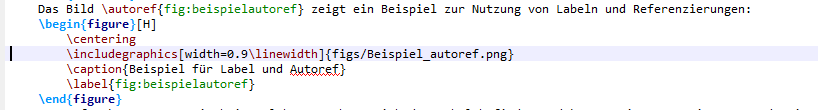
\includegraphics[width=1.0\linewidth]{figs/Beispiel_autoref.png}
		\caption{Beispiel für Label und Autoref}
		\label{fig:beispielautoref}
	\end{figure}
	Autoref erkennt automatisch in welcher Umgebung sich das Label befindet und kennt seine Nummerierung. Zudem ist diese Referenzierung im PDF anklickbar und man gelangt direkt zu dem Teil, wo das Label gesetzt wurde.\newline\newline
	
	Für Quellen wird der folgende Befehl verwendet:
	\begin{verbatim}
		\cite[postnote]{bibid}
	\end{verbatim}
	Bibid ist der Name der Quelle aus der "sources.bib", also die verwendete Quelle.\newline
	Als postnote kann zum Beispiel S22-25 eingetragen werden.
	
	
	
	\newpage
	\section{Inkscape Latex}
	
	
	
	
	\newpage
	\section{Bilder}
	\subsection{Bild einfügen}
	Um ein Bild einzufügen kann dies händisch mit nachfolgendem geschehen oder in TeXstudio $\rightarrow$ "Assistenten" $\rightarrow$ "Grafik Einfügen" als Hilfe genutzt werden.
	\begin{verbatim}
		\begin{figure}[H]
			\centering
			\includegraphics[width=0.7\linewidth]{ORDNER/BILDNAME.DATEIFORMAT}
			\caption{BILDUNTERSCHRIFT}
			\label{fig:LabelName}
		\end{figure}
	\end{verbatim}
	Das \text{[H]} steht für "here", das Bild wird also genau an der Stelle eingefügt, wo auch der Code in Latex steht. Ansonsten erscheint das Bild immer ganz oben im PDF.\newline
	"Centering" ist um das Bild zu zentrieren.\newline
	"includegraphics" importiert das Bild. Dabei ist darauf zu achten, dass der Pfad, Dateiname und das Dateiformat richtig eingetragen sind. In dieser Vorlage sind Ordner wie "figs" und "Bilder" bereits Standardpfade und müssen nicht angegeben werden.\newline
	Die Größe kann mit "width=" verändert werden.\newline
	"Caption" ist die Bildunterschrift, also der Text unter dem Bild, welcher im PDF erscheint.
	"Label" sollte bereits bekannt sein. Mit diesem Namen kann auf das Bild referenziert werden. Zur Kennzeichnung ist es üblich, dass Labels für Bilder mit "fig:" beginnen und dahinter der Name kommt.
	\subsection{Platzhalter für nachträgliche Bilder}
	Platzhalter dienen dazu, noch nicht fertige/vorhandene Bilder mit einem Achtungszeichen zu integrieren. So hat man das Label, kann damit weiterarbeiten und denkt später daran, das Bild noch hinzuzufügen und muss nur eine Kleinigkeit ändern.
	\begin{verbatim}
		\begin{figure}[H]
			\centering
			\missingfigure{TEXT ZUR BESCHREIBUNG WAS FEHLT}
			\captionof{figure}{BILDUNTERSCHRIFT}
			\label{fig:LABEL}
		\end{figure}
	\end{verbatim}
	In "missingfigure" kann ein kleiner Text zur Beschreibung was genau Fehlt. Dieser erscheint auch im PDF.



	
	
	\newpage
	\section{Einfache Tabellen}




	
	\newpage
	\section{Mathe- Formelumgebung}
	\subsection{Formeln}
	\subsubsection{Einzelne Formeln}
	Um einfache Mathematische Formeln in den Text einzubinden gibt es folgende Umgebung:
	\begin{verbatim}
		\begin{equation}
			Inhalt...
		\end{equation}
	\end{verbatim}
	Bei dieser wird die Nummerierung automatisch normgerecht angepasst. Die Gleichung kann zusätzlich mit einem Label versehen werden und auf diese mittels autoref im Text verwiesen werden. Für einfache Unterscheidung sollten Label für Gleichungen immer mit "eq:" beginnen.
	\subsubsection{Mehrere Formeln gleicher Nummerierung}
	Hat man mehrere Gleichungen, welche die gleiche Nummer erhalten sollen und nur durch a) b) c)... unterschieden werden funktioniert dies mit folgender Umgebung:
	\begin{verbatim}
		\begin{subequations}
			\begin{align}
				&Gleichung 1\\
				&Gleichung 2\\
				&Gleichung 3
			\end{align}
		\end{subequations}
	\end{verbatim}
	Jede neue Gleichung beginnt mit einem \& und endet mit \\\\ für einen Zeilenumbruch zur nächsten Formel. Die letzte erhält kein \\\\ Ansonsten entsteht eine weitere Formel ohne Inhalt! \newline
	Jede einzelne der Subequations kann mit einem Label versehen werden.
	\subsubsection{Zeilenumbruch innerhalb einer Formel}
	Für längere Formeln, welche nicht in eine Zeile passsen gibt es folgende Möglichkeit:
	\begin{verbatim}
		\begin{equation} 
			\begin{split} 
				Zeile1 &= Zeile1 \\ 
				Zeile2 &= Zeile2
			\end{split} 
		\end{equation} 
	\end{verbatim}
	Der Vorteil des \&= ist, dass die Zeilen nach dem "=" ausgerichtet sind untereinander. Es gibt auch die "multiline" Umgebung, allerdings ist dort die zweite Zeile Linksbündig, was nicht gut aussieht.
	
	\subsection{Vektoren und Matrizen}
	\subsubsection{Vektoren}
	\subsubsection{Matrizen}
	
	\subsection{Sonderzeichen}
	
	
	
	\newpage
	\section{SI}
	
	
	
	
	\newpage
	\section{Komplexere Tabellen}
	\begin{verbatim}
		\begin{table}[H]
			\centering
			\captionof{table}{Tabellenüberschrift}
			\renewcommand{\arraystretch}{2} % Senkrechten Abstand für diese Tabelle erhöhen
			\setlength{\tabcolsep}{0.3em} % Horizontalen Abstand für diese Tabelle erhöhen
			% S in table richtet diese nach kommata aus
			% dies funktioniert bei starkunsymetreischen zahlen nicht.
			% dazu kann man mit table-format = A.B die anzahl der erwarteten stellen eingeben 
			dabei steht A für die Anzahl der zahlen vor dem komma und B fur die Anzahl hinter 
			dem komma
			% test in der spalte mit {} umklammern bsp {text $P_A$}
			
			% \makecell{ 1. zeile \\ 2. zeile} ermögtlicht einfache zeilenumbrüche in einer zelle
			\begin{tabular}{|c|c|S[ table-format = 2.3]|S[ table-format = 2.3]|
					S[ table-format = 1.4]|S[ table-format = 1.4]|}
				\hline
				\multicolumn{2}{|c|}{}& {\makecell{Ergebnis\\ der Wirkleistung \\ 
						aus der Simulation \\ in Watt}} & {\makecell{berechnete \\
						Wirkleistung\\ in Watt}} &{Abweichungen} 
					    &{\makecell{Abweichung\\ in \%}} \\ \hline
				\multirow{3}{*}{\makecell{$L_1$\\ als Bezug}} 
				&  $P_A$ & 15,500 & 15,4954 & 0,0046 & 0,0297 \\ \cline{2-6} 
				& $P_B$ & 47,761 & 47,7607 & 0,0003 & 0,0006 \\ \cline{2-6} 
				& $P_{ges}$ & 63,261 & 63,2561 & 0,0049 & 0,0077 \\ \hline
				\multirow{3}{*}{\makecell{$L_2$ \\als Bezug}}
				& $P_A$ & 38,398 & 38,3972 & 0,0008 & 0,0021 \\ \cline{2-6} 
				& $P_B$ & 24,863 & 24,8624 & 0,0006 & 0,0024 \\ \cline{2-6} 
				& $P_{ges}$ & 63,261 & 63,2596 & 0,0014 & 0,0022 \\ \hline
			\end{tabular}
		\end{table}
	\end{verbatim}
	Dieser Code entspricht folgender Tabelle:
		\begin{table}[H]
		\centering
		\captionof{table}{Tabellenüberschrift}
		\renewcommand{\arraystretch}{2} % Senkrechten Abstand für diese Tabelle erhöhen
		\setlength{\tabcolsep}{0.3em} % Horizontalen Abstand für diese Tabelle erhöhen
		% S in table richtet diese nach kommata aus
		% dies funktioniert bei starkunsymetreischen zahlen nicht.
		% dazu kann man mit table-format = A.B die anzahl der erwarteten stellen eingeben 
		%dabei steht A für die Anzahl der zahlen vor dem komma und B fur die Anzahl hinter 
		%dem komma
		% test in der spalte mit {} umklammern bsp {text $P_A$}
		
		% \makecell{ 1. zeile \\ 2. zeile} ermögtlicht einfache zeilenumbrüche in einer zelle
		\begin{tabular}{|c|c|S[ table-format = 2.3]|S[ table-format = 2.3]|
				S[ table-format = 1.4]|S[ table-format = 1.4]|}
			\hline
			\multicolumn{2}{|c|}{}& {\makecell{Ergebnis\\ der Wirkleistung \\ 
					aus der Simulation \\ in Watt}} & {\makecell{berechnete \\
					Wirkleistung\\ in Watt}} &{Abweichungen} 
			&{\makecell{Abweichung\\ in \%}} \\ \hline
			\multirow{3}{*}{\makecell{$L_1$\\ als Bezug}} 
			&  $P_A$ & 15,500 & 15,4954 & 0,0046 & 0,0297 \\ \cline{2-6} 
			& $P_B$ & 47,761 & 47,7607 & 0,0003 & 0,0006 \\ \cline{2-6} 
			& $P_{ges}$ & 63,261 & 63,2561 & 0,0049 & 0,0077 \\ \hline
			\multirow{3}{*}{\makecell{$L_2$ \\als Bezug}}
			& $P_A$ & 38,398 & 38,3972 & 0,0008 & 0,0021 \\ \cline{2-6} 
			& $P_B$ & 24,863 & 24,8624 & 0,0006 & 0,0024 \\ \cline{2-6} 
			& $P_{ges}$ & 63,261 & 63,2596 & 0,0014 & 0,0022 \\ \hline
		\end{tabular}
	\end{table}




	\newpage
	\section{Programmiercode}
	
	
	
	
	\newpage
	\section{Fehlermeldungen}
	
	
	\newpage
	\printbibliography
	
\end{document}
